% Options for packages loaded elsewhere
\PassOptionsToPackage{unicode}{hyperref}
\PassOptionsToPackage{hyphens}{url}
%
\documentclass[
]{article}
\usepackage{lmodern}
\usepackage{amssymb,amsmath}
\usepackage{ifxetex,ifluatex}
\ifnum 0\ifxetex 1\fi\ifluatex 1\fi=0 % if pdftex
  \usepackage[T1]{fontenc}
  \usepackage[utf8]{inputenc}
  \usepackage{textcomp} % provide euro and other symbols
\else % if luatex or xetex
  \usepackage{unicode-math}
  \defaultfontfeatures{Scale=MatchLowercase}
  \defaultfontfeatures[\rmfamily]{Ligatures=TeX,Scale=1}
\fi
% Use upquote if available, for straight quotes in verbatim environments
\IfFileExists{upquote.sty}{\usepackage{upquote}}{}
\IfFileExists{microtype.sty}{% use microtype if available
  \usepackage[]{microtype}
  \UseMicrotypeSet[protrusion]{basicmath} % disable protrusion for tt fonts
}{}
\makeatletter
\@ifundefined{KOMAClassName}{% if non-KOMA class
  \IfFileExists{parskip.sty}{%
    \usepackage{parskip}
  }{% else
    \setlength{\parindent}{0pt}
    \setlength{\parskip}{6pt plus 2pt minus 1pt}}
}{% if KOMA class
  \KOMAoptions{parskip=half}}
\makeatother
\usepackage{xcolor}
\IfFileExists{xurl.sty}{\usepackage{xurl}}{} % add URL line breaks if available
\IfFileExists{bookmark.sty}{\usepackage{bookmark}}{\usepackage{hyperref}}
\hypersetup{
  pdftitle={Sensitivity Analysis},
  hidelinks,
  pdfcreator={LaTeX via pandoc}}
\urlstyle{same} % disable monospaced font for URLs
\usepackage[margin=1in]{geometry}
\usepackage{longtable,booktabs}
% Correct order of tables after \paragraph or \subparagraph
\usepackage{etoolbox}
\makeatletter
\patchcmd\longtable{\par}{\if@noskipsec\mbox{}\fi\par}{}{}
\makeatother
% Allow footnotes in longtable head/foot
\IfFileExists{footnotehyper.sty}{\usepackage{footnotehyper}}{\usepackage{footnote}}
\makesavenoteenv{longtable}
\usepackage{graphicx,grffile}
\makeatletter
\def\maxwidth{\ifdim\Gin@nat@width>\linewidth\linewidth\else\Gin@nat@width\fi}
\def\maxheight{\ifdim\Gin@nat@height>\textheight\textheight\else\Gin@nat@height\fi}
\makeatother
% Scale images if necessary, so that they will not overflow the page
% margins by default, and it is still possible to overwrite the defaults
% using explicit options in \includegraphics[width, height, ...]{}
\setkeys{Gin}{width=\maxwidth,height=\maxheight,keepaspectratio}
% Set default figure placement to htbp
\makeatletter
\def\fps@figure{htbp}
\makeatother
\setlength{\emergencystretch}{3em} % prevent overfull lines
\providecommand{\tightlist}{%
  \setlength{\itemsep}{0pt}\setlength{\parskip}{0pt}}
\setcounter{secnumdepth}{-\maxdimen} % remove section numbering

\title{Sensitivity Analysis}
\author{}
\date{\vspace{-2.5em}3 December 2020}

\begin{document}
\maketitle

\hypertarget{approach}{%
\subsection{Approach}\label{approach}}

For this example it is assumed that the output variables of interest are
`Foyer Max Heat FED' and `Foyer Heat FED'. Notionally, we might say that
we are interested in the amount of time people have to escape (represented
by the time during which they foyer--through which they must
evacuate--remains viable) and the worst temperature they might have to
face in the Foyer during that evacuation.

Sensitivity analysis is interested in the sensitivity the output has to
each input. This is typically expressed in terms of the percent
variation in output produced by a one percent variation in each input.
As it turns out, simple linear regression of the \emph{log} of the
inputs against the \emph{log} of the output will give exactly that
value.

The second target variable--Foyer Heat FED--was selected to illustrate
an additional complication in the analysis. This variable expresses the
time till the FED reaches the value of 1--assumed to represent the
condition where the space is no longer viable. The complication is that
in a number of cases nonviability does not occur within the time of the
simulation: here some 89.7~\% of cases do not result in non-viability.
That presents a problem because analyzing the data without taking that
into account will result in incorrect estimates of the sensitivity.

In this case what is run is a `Tobit' analysis\footnote{Tobin, James
  (1958). ``Estimation of Relationships for Limited Dependent
  Variables.'' Econometrica. 26 (1): 24--36. \url{doi:10.2307/1907382}.}
which properly accounts for the effect of the cases where non-viability
did not occur. The `Tobit' analysis is also performed on a log-log
transformation of the data.

\hypertarget{number-of-cases}{%
\section{Number of Cases}\label{number-of-cases}}

An initial run of 1000 cases was evaluated. The chart below shows the
coefficient for \texttt{Lab\_depth} for the first model as a function of
the number of cases. Examination of the chart shows that the value for
the coefficient is still changing substantially at the end of 1000
cases. When the number of cases were increased to 2500 the results still
did not seem very stable. When the cases increased again to 5000 there
was a noticeable trend over the last thousand or so cases. When the
cases were increased to 10~000, the estimated value over the last couple
of thousand cases seems to have settled down. So these results are based
on 10~000 cases.

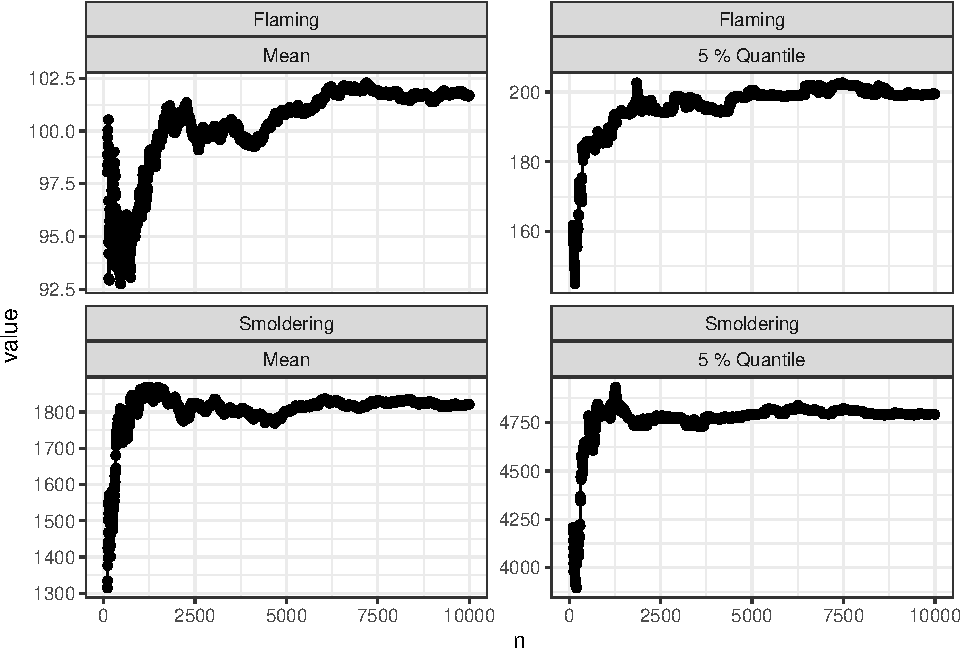
\includegraphics{Sensitivity_files/figure-latex/cvg_plot-1.pdf}

\hypertarget{discussion}{%
\section{Discussion}\label{discussion}}

First we look at the sensitivity of maximum temperature FED in the
Foyer. Selected results are displayed in Table 1. The single most
significant factor is the depth of the lab space--where the fire
occurred. A one-percent change in the lab depth will produce a 0.53~\%
decrease in the maximum heat FED for the Foyer. Similarly a one percent
change in the height of the Foyer and halls produces a 0.47~\% decrease
in the heat FED for the Foyer. At the other end of the scale changes in
the Foyer width or the depth of office 1 produce minimal changes to the
heat FED for the Foyer.

\begin{longtable}[]{@{}lrrrrc@{}}
\toprule
& Value & Std. Error & t value & Pr(\textgreater\textbar t\textbar)
&\tabularnewline
\midrule
\endhead
log(Lab\_depth) & -0.5328 & 0.16 & -3.33 & 0.0009 & ***\tabularnewline
log(Front\_Hall\_depth) & 0.1206 & 0.16 & 0.75 & 0.4551 &\tabularnewline
log(Foyer\_width) & 0.0053 & 0.16 & 0.03 & 0.9735 &\tabularnewline
log(\texttt{Office\_\#1\_depth}) & -0.0042 & 0.16 & -0.03 & 0.9791
&\tabularnewline
log(\texttt{Office\_\#2\_height}) & 0.4525 & 0.16 & 2.84 & 0.0045 &
**\tabularnewline
log(Foyer\_and\_Halls\_height) & -0.4661 & 0.16 & -2.94 & 0.0033 &
**\tabularnewline
log(FrontHall2EvenHall\_WIDTH) & -0.0054 & 0.16 & -0.03 & 0.9727
&\tabularnewline
log(Gyp\_Emissivity.1) & 0.1223 & 0.16 & 0.76 & 0.4458 &\tabularnewline
log(\texttt{Ofice\_\#4\_\_Door\_Height}) & -0.0029 & 0.16 & -0.02 &
0.9856 &\tabularnewline
log(\texttt{Ofice\_\#6\_\_Door\_Height}) & 0.1209 & 0.16 & 0.75 & 0.4512
&\tabularnewline
log(Fire\_HRR\_scaling\_factor) & 0.0398 & 0.16 & 0.25 & 0.8051
&\tabularnewline
log(Fire\_time\_scaling\_factor) & -0.3920 & 0.16 & -2.45 & 0.0141 &
*\tabularnewline
\bottomrule
\end{longtable}

In Table 2, we look at just those variables for which a one-percent
change produces a change of greater than 0.2~\% in the time to
non-viability for the Foyer, plus the scaling factors for the fire.
Those variables include variables related to the room of fire origin
(Lab\_depth), factors related to the space itself (Foyer\_width,
Front\_Door\_Width), factors related to the spaces through which the
fire must travel (Even\_Hallway\_depth, Odd\_Hallway\_width,
Front\_Hall\_depth) and some additional miscellaneous factors
(Office\_.2\_height Office\_.5\_height Gyp\_Conductivity.1
Gyp\_Density.1).

\begin{longtable}[]{@{}lrrrrc@{}}
\toprule
& Value & Std. Error & t value & Pr(\textgreater\textbar t\textbar)
&\tabularnewline
\midrule
\endhead
log(Lab\_depth) & 0.3460 & 0.14 & 2.40 & 0.0162 & *\tabularnewline
log(Even\_Hallway\_depth) & 0.3043 & 0.14 & 2.12 & 0.0341 &
*\tabularnewline
log(Odd\_Hallway\_width) & 0.2359 & 0.14 & 1.64 & 0.1011
&\tabularnewline
log(Front\_Hall\_depth) & -0.2318 & 0.15 & -1.59 & 0.1116
&\tabularnewline
log(Foyer\_width) & -0.2778 & 0.15 & -1.91 & 0.0555 & .\tabularnewline
log(\texttt{Office\_\#2\_height}) & -0.2103 & 0.14 & -1.46 & 0.1431
&\tabularnewline
log(\texttt{Office\_\#5\_height}) & 0.2564 & 0.14 & 1.78 & 0.0753 &
.\tabularnewline
log(Gyp\_Conductivity.1) & 0.2454 & 0.14 & 1.70 & 0.0889 &
.\tabularnewline
log(Gyp\_Density.1) & 0.2217 & 0.14 & 1.54 & 0.1233 &\tabularnewline
log(Front\_Door\_Width) & 0.3057 & 0.14 & 2.13 & 0.0333 &
*\tabularnewline
log(Fire\_HRR\_scaling\_factor) & -0.0462 & 0.15 & -0.32 & 0.7510
&\tabularnewline
log(Fire\_time\_scaling\_factor) & 0.1927 & 0.14 & 1.34 & 0.1790
&\tabularnewline
\bottomrule
\end{longtable}

\end{document}
